\documentclass[letterpaper]{article}

% Parts of the style depend on whether a PDF or a DVI output is created.
\usepackage{ifpdf}

\usepackage{aaai}
\usepackage{amsfonts}
\usepackage{amsmath}
\usepackage{amsthm}
\usepackage{courier}
\usepackage[english]{babel}

% Include graphics.
\usepackage{graphicx}
\ifpdf
  % Declare the supported file extensions.
  \DeclareGraphicsExtensions{.jpg,.mps,.pdf,.png}
\fi

\usepackage{helvet}
\usepackage[utf8]{inputenc}
\usepackage{times}
\usepackage{verbatim}
\usepackage{changebar}
\usepackage[normalem]{ulem}
\usepackage{url}
\newcommand{\URL}[1]{{\small \url{#1}}}

% Operator macros.
\newcommand{\absolute}[1]{\lvert#1\rvert}
\newcommand{\bigsetdef}[2]{\big\{#1\,\,\big\vert\,\,#2\big\}}
\newcommand{\card}[1]{\lvert#1\rvert}
\newcommand{\equivpair}[2]{#1 \approx #2}
\newcommand{\equivset}[1]{[#1]_{\approx}}
\newcommand{\higherapprox}[0]{\overline{\approx}}
\newcommand{\interp}[1]{#1^{\mathcal{I}}}
\newcommand{\lowerapprox}[0]{\underline{\approx}}
\newcommand{\natnum}[1]{#1 \in \mathbb{N}}
\newcommand{\pair}[2]{\langle#1,#2\rangle}
\newcommand{\powerset}[1]{\mathcal{P}(#1)}
\newcommand{\range}[2]{#1,\ldots,#2}
\newcommand{\set}[1]{\{#1\}}
\newcommand{\setdef}[2]{\{#1\,\vert\,#2\}}
\newcommand{\setrange}[2]{\{#1,\ldots,#2\}}
\newcommand{\triple}[3]{\langle#1,#2,#3\rangle}
\newcommand{\tuple}[1]{\langle#1\rangle}
\newcommand{\tuplerange}[2]{\langle#1,\ldots,#2\rangle}

% Operator declarations
\DeclareMathOperator{\indpo}{{\mathbb{IND}-\mathbb{PO}}}
\DeclareMathOperator{\indp}{{\mathbb{IND}-\mathbb{P}}}

% Theorem styles.
\newtheorem{assumption}{Assumption}
\newtheorem{axiom}{Axiom}
\newtheorem{convention}{Convention}
\newtheorem{example}{Example}
\newtheorem{definition}{Definition}
\newtheorem{lemma}{Lemma}
\newtheorem{principle}{Principle}
\newtheorem{proposition}{Proposition}
\newtheorem{specification}{Specification}
\newtheorem{statement}{Statement}
\newtheorem{theorem}{Theorem}
%\theoremstyle{definition}

\frenchspacing

\setlength{\pdfpagewidth}{8.5in}
\setlength{\pdfpageheight}{11in}

\pdfinfo{
/Title Rough Set Semantics for Identity on the Web
/Author Wouter Beek, Stefan Schlobach, Frank van Harmelen}
\setcounter{secnumdepth}{1}

\author{
  Wouter Beek \and Stefan Schlobach \and Frank van Harmelen\\
  Vrije Universiteit Amsterdam\\
  De Boelelaan 1081a\\
  1081HV Amsterdam\\
  The Netherlands
}

\title{Rough Set Semantics for Identity on the Web}

\begin{document}

\maketitle
\begin{abstract}
Identity relations are at the foundation of many
  logic-based knowledge representations.
We argue that the traditional notion of equality,
  based on Leibniz' principle of indiscernability,
  is unsuited for many realistic knowledge representation settings.
The classical  interpretation of equality is simply too strong
  when the equality statements are re-used outside their original context.

The most prominent modern example of such re-use of knowledge across contexts
  is the Linked Open Data initiative, and the Semantic Web in general.
On the Semantic Web, equality statements are used to interlink
  multiple descriptions of the same object,
  using {\small \texttt{owl:sameAs}} assertions.
And indeed, many practical uses of {\small \texttt{owl:sameAs}}
  are known to violate the formal Leibniz-style semantics.

First, we survey the problems with the classical definition of identity,
  both in general, and on the Semantic Web in particular. 
In order to provide a more flexible semantics to identity,
  we then propose a method that assigns meaning to the subrelations of
  an identity relation using the predicates that are used in a knowledge-base.
Using those indiscernability-predicates,
  we define upper and lower approximations of equality in the style of
  rought-set theory, resulting in a quality-measure for
  the identity relation.

We illustrate our approach on a realistic Semantic Web dataset,
  and we experimentally verify that our approach yields
  the intuitively desired results on this dataset.

%The full code and results of our experiments are available at
%  \URL{wouterbeek.com/identity-on-the-web} and
%  \URL{github.com/wouterbeek/IOTW}.



\end{abstract}

\section{Introduction}
\label{sec:intro}
\label{sec:relwork}

Clustering resources into different kinds can be useful
 for various purposes, e.g. browsing based on categories,
 providing automatic suggestions for ontology design.

We argue that RDF data deals with resources of different ``kinds'':
 two resources of the same kind will have similar relations
 to other resources.
We exploit this to partition the data into ``kinds'' automatically.

There are various ways to partition a set of resources into kinds.
The most straightforward approach is to use an explicit vocabulary
 in order to indicate
   that resources are members of the same set (extensional definition)
 or
   that resources are instance of the same class (intensional definition).
The vocabulary of RDF(S) \cite{BrickleyGuha2014} uses
 the intensional definition,
 denoted by the \texttt{rdf:type} property term.

In addition to used the explicit schema information,
 various methods have been explored that
 extract implicit schema information.
In \cite{NeumannMoerkotte2011},
 kinds of resources are identified
 by their \emph{characteristic set},
 which is the set properties that are asserted of a resource.

A comparison of the type-based and the property-based
 identification of resource kinds was performed by \cite{GottronKSS13},
 who showed that there is considerable mutual information between
 these two approaches.

A third approach is to use the object terms in addition to the predicate terms
 in order to characterize a resource.
In \cite{buikstra2011ranking}, the similarity between two resources
 is measured by the number of predicate-object pairs they have in common.

As we will argue in Section \ref{sec:fingerprints},
 the existing approaches towards partitioning a set of resources
 have shortcomings: they either identify too few partition members
 given the data at hand, or they identify too many partition members
 than can be substantiated by the data. 

In Section \ref{sec:approach} we give a generalization of
 these existing approaches and show that for arbitrary datasets
 more granular partitions can be found that are still validated
 by the data, i.e. that do not overfit.
Section \ref{sec:implementation} gives some implementation details,
 and Section \ref{sec:evaluation} shows the evaluation results we
 obtained by executing our implementation on existing datasets.
Section \ref{sec:conclusion} concludes.


\section{Stating the problem}
\label{sec:stating_the_problem}

Identity is often understood as the sharing of all properties between
  two objects with different names. 
This statement is known as the principle of indiscernibility
  (see principle \ref{principle:indiscernibility_of_identicals})
  and has been attributed to Leibniz \cite{Forrest2010}.\footnote{
    Inverting the implication in
      principle \ref{principle:indiscernibility_of_identicals}
      results in the identity of indiscernibles,
      which is trivially true since identity with $\phi(b)$
      is one of the properties.
    }
% According to Forrest2010 this can be found in Gottfried Wilhelm Leibniz,
% Discourse on Metaphysics, section 9.
% There I find the following passage:
% \begin{quote}
% That every individual substance expresses the whole universe
%   in its own manner and that in its full concept is included
%   all its experiences together with all the attendant circumstances
%   and the whole sequence of exterior events.
% \end{quote}

\begin{principle}[Indiscernibility of identicals]
\label{principle:indiscernibility_of_identicals}
\begin{equation}
    a = b
  \rightarrow
    \forall \phi \in \Phi (\phi(a) = \phi(b)\nonumber)
\end{equation}
\end{principle}

\noindent Although the principle provides necessary and sufficient conditions
  for identity, it does not point toward an automated procedure
  for enumerating the extension of the identity relation.
Due to its circular nature, the set of properties includes
  ``being identical to $x$'' (for every object $x$).
Even though this principle does not
  allow a positive identification of identity pairs,
  it does provide an exclusion condition;
  namely objects that are known to not share some property
  are also known to not be identical.

\subsection{Generic problems of identity}

Identity poses several problems that are not specific to the SW.
Firstly, identity does not hold across (all) modal contexts,
  allowing Lois Lane to believe that Superman saved her,
  without knowing that Clark Kent saved her.

Secondly, identity seems to be a context-specific concept \cite{Geach1967},
  allowing two medicines to be the same chemical substance
  while not being the same commercial drug.

Thirdly, identity over time poses problems,
  since a ship may be considered the same
  even though all the components from which it is built
  have been changed over the course of time \cite{Lewis1986}.

Lastly, there is the problem of identity under counterfactual assertions
  such as ``If Obama would have been born outside the US,
  then he would not have been president of the US today.''\cite{Kripke1980}

\subsection{SW-specific problems of identity: Semantics}

Besides the generic problems of identity,
  there are problems specific to the SW.
The first SW-specific problem follows from its semantics;
  the second follows from its pragmatics.
The semantics for SW identity are given in definition \ref{def:owl_sameAs}.

\begin{definition}[Semantics of {\small \texttt{owl:sameAs}}]
\label{def:owl_sameAs}
\begin{equation}
    \langle a, b \rangle \in Ext(I({\small \texttt{owl:sameAs}}))
  \,\iff\,
    a = b\nonumber
\end{equation}
\end{definition}

\noindent In the context of the SW,
  identity assertions are extra strong because of the Open World Assumption.
Stating that two objects are the same
  implies that from now on no new property can be stated about
  only one of those objects
  (this follows from definition \ref{def:owl_sameAs} in combination with
  the principle of substitutivity \emph{salva veritate}).
  % Look this one up in
  % W.V.O. Quine, Quintessence, extensions, Reference and Modality, p. 378.
  % Looked this one up, interesting, but is not directly applicable here.
For instance, when one SW contributor claims that
  medicines $a$ and $b$ are the same
  based on them having the same chemical composition,
  this prohibits another SW contributor from stating that
  $a$ and $b$ are produced by different companies
  without her introducing an inconsistency.
Formulated in terms of
  principle \ref{principle:indiscernibility_of_identicals},
  on the SW the set $\Phi$ contains
  all properties that can possibly be expressed
  in the modeling language.
This set is obviously much bigger than the actual vocabulary
  of any in-use dataset.

Moreover, whether or not two objects share the absence of a property
  (i.e., a property of the form ``does not have the property $\phi$''),
  cannot be concluded based on the absence of a property assertion.
Such `negative knowledge' must be provided explicitly
  using class restrictions.

\subsection{SW-specific problems of identity: Pragmatics}

When we take the social component of the SW into account,
  we observe that modelers have different opinions about
  whether two objects are identical or not,
  because they operate in different contexts.
This is unlike many traditional uses of knowledge-bases,
  where a knowledge-base is rarely re-used outside its original
  context of construction.
As a consequence, SW modelers are known not to conform to
  the strict semantics of identity (definition \ref{def:owl_sameAs}),
  resulting in situations where one person
  claims two objects are identical
  whereas another considers them to be only (closely) related.
It is indeed unrealistic that all who contribute to the SW
  are able to quantify over the entire realm of possible properties
  (i.e., $\Phi$ in principle \ref{principle:indiscernibility_of_identicals}).

The SW community recognizes this tension between
  the semantics and pragmatics of identity.
At the Semantics for Big Data track at the AAAI Fall Symposium 2013
  \cite{SemanticsBigData2013}
  the problem of identity was considered one of the most
  pressing problems facing the Semantic Web today.

The pragmatics of the SW is encoded in the open-ended collection of
  common practices that effectuate the creation and usage of SW content.
An example of such an encoded common practice is the five `stars'
  of Linked Open Data (LOD) publishing \cite{Bernerslee2010}.
These five `stars' are effectively five \emph{maxims} that specify
  (part of) the pragmatics of LOD publishing,
  much like the Gricean maxims specify
  (part of) the pragmatics of natural language discourse \cite{Grice1989}.
The fifth `star' or maxim is given in \ref{eq:data_linking_maxim}.
\begin{principle}[Data linking maxim]
  \label{eq:data_linking_maxim}
  \begin{quote}
    Link your data to other people's data to provide context.
  \end{quote}
\end{principle}

\noindent Given that RDF links are often specified by using
  the {\small \texttt{owl:saveAs}} predicate term \cite{Void2011}
  % The VoID W3C Interest Group Note states that
  % ``RDF links often have the \texttt{owl:sameAs} predicate.''
  we conclude that the pragmatics of the SW
  aggravates the already problematic semantics of identity.

The pragmatics of the SW, observed in contemporary common practices,
  states that by asserting identity between objects,
  more context is added for those objects,
  since such identity links result in more facts being asserted
  about the same resource.
At the same time we see that the strict semantics of identity
  gets violated once the context in which an object was created
  is extended -- by identity assertions -- beyond its original context
  (see the section on the generic problems of identity).
This is true regardless of whether `context' is defined in terms of
  `intended use', `domain', `time', or `modality'.

Concluding, from the social point of view the requirements on SW modelers
  are unreasonably high when they are required to
  assert identity links in accordance with the semantics.
At the same time the pragmatics states that modelers should
  make those links in order to place their knowledge into context.



\subsection{Research goals}
\label{sec:research_goals}

Based on the above analysis, we can state the following desiderata for 
an identity relation that does not suffer from the problems stated above: 

\begin{enumerate}
\item In an identity relation the pairs all look the same.
      We want to characterize subrelations of an identity relation in terms
      of the predicates that are important in a particular context.
\item Based on an existing identity relation we want to give semantically
      motivated suggestions for extending or limiting the identity relation.
\item We want to assess the quality of an identity relation based on
      the consistency with which it is applied to the data.
\end{enumerate}

\section{Related work}
\label{sec:related_work}

Existing research suggests six different solutions for
  the problem of identity on the SW.

\textbf{[1] Introduce weaker versions of {\small \texttt{owl:sameAs}}}
  \cite{HalpinHayes2010,MccuskerMcguinness2010}.
Candidates for replacement are
  the SKOS concepts
  {\small \texttt{skos:related}} and {\small \texttt{skos:exactMatch}}
  \cite{MilesBechhofer2009}.
The former is not transitive,
  thereby limiting the possibilities for reasoning.
The latter is transitive,
  but can only be used in certain contexts.
It is not defined in what contexts it can be used
  \cite{MilesBechhofer2009}.\footnote{
    For instance, the property {\small \texttt{skos:exactMatch}}
    ``is used to link two concepts, indicating a high degree of confidence
    that the concepts can be used interchangeably across a wide range of
    information retrieval applications.''
  }
\begin{comment}
% SIMILARITY
The problem with using weaker notions such as relatedness,
  is that everything is related to everything in \emph{some} way.}
% Shall we discuss similarity here as well?
% Does similarity differ from relatedness?
\end{comment}

\textbf{[2] Restrict the applicability of identity relations}
  to specific contexts.
In terms of Semantic Web technology, identities are expected to hold
  within a named graph or within a namespace,
  but not necessarily outside of it \cite{HalpinHayes2010}.
\cite{Melo2013} has successfully used the Unique Names Assumption
  within namespaces in order to identify many (arguably) spurious
  identity statements.

\textbf{[3] Introduce additional vocabulary} that does not weaken but extends
  the existing identity relation.
\cite{HalpinHayes2010} mention an explicit distinction that could be made
  between mentioning a term and using a term,
  thereby distinguishing an object and a Web document describing that object.
Other possible extensions of {\small \texttt{owl:sameAs}} might take
  the Fuzzyness and/or uncertainty of identity statements into account.

\textbf{[4] Use domain-specific identity relations}
  \cite{MccuskerMcguinness2010}.
For instance
    ``$x$ and $y$ have the same medical use''
  replaces
    identity in the domain of medicine,
and
    ``$x$ and $y$ are the same molecule''
  replaces
    identity in the domain of chemistry.
The downside to this solution is that domain-specific links are
  only locally valid, thereby limiting knowledge reuse.

\textbf{[5] Change the modeling practice}, possibly in a (semi-)automated way
  by adapting visualization and modeling toolkits to produce notifications
  upon reading SW data, or by posing additional restrictions on the creation
  and alteration of data. For example, adding an RDF link could require
  reciprocal confirmation from the maintainers of the respective datasets.
  \cite{HalpinHayes2010,DingShinavierFininMcguinness2010}
The problem with introducing checks on editing operations,
  is that it violates one of the fundamental underpinnings of the SW;
  namely that on the Web of Data anybody is allowed to say
  anything about anything \cite{AntoniouGrothHarmelenHoekstra2012}.

\textbf{[6] Extract network properties of {\small \texttt{owl:sameAs}}
  datasets} \cite{DingShinavierShangguanMcguinness2010}.
Although this work shows that network analysis can provide insights
  into the ways in which identity is used in the SW,
  these endeavors have not yet been related to the semantics of the
  identity relation.
We believe that utilizing network theoretic aspects in order to
  determine the meaning of identity statements
  would be interesting future research.

What the existing approaches have in common is
  that quite some work has to be done
  (adapting or creating standards, instructing modelers, converting existing
  datasets) in order to resolve only some of the problems of identity.
Our approach provides a way of dealing with the heterogeneous real-world
  usage of identity in the SW that is fully automated and requires
  no changes to standards, modeling practices, or existing datasets.


\section{Approach}
\label{sec:approach}

In contrast to the explicit schema information that should be present
in an RDF data set in the form of \texttt{rdf:type} specifications, in
this section we will use the structural properties of the graph to
extract implicit schema information.
structural properties of the graph can be used

In the previous section we saw that both excluding and including object terms
 in the partitioning of resources has negative effects on some data.
In this section we seek the best of both worlds
 and generalize these approaches using a partition $\M$ of resources.

Let $\tn{class}(t) = C$ iff $t \in C$ and $C \in \M$,
 thus the class of a term is its partition cell.
We now define the generic fingerprint (called $f_\M$) of a subject term $s$
 in Definition \ref{def:fingerprint}.

\begin{definition}[Fingerprint]
  \label{def:fingerprint}
  $
    f_\M(s)
  := \\
    \{
      \tuple{p,C} \in P_G \times \mathcal{P}(O_G)
    \mid
      \pair{I(s)}{I(o)} \in Ext(I(p)) \, \wedge \, o \in C \\
      \wedge \, C \in \M
    \}
  $
\end{definition}

The fingerprints $f_2$ and $f_3$ in Section \ref{sec:fingerprints}
 are instantiations of the generic fingerprint $f_\M$.
They correspond to, respectively,
  a partition $\M$ that contains a single set of all terms,
 and
  a partition $\M$ that contains all terms as singleton sets.

The advantage of generalizing these methods using $f_m$ is that
 a well chosen $\M$ can interpolate between these two existing approaches,
 and retain all relevant information about the term while discarding
 irrelevant details.
Our method of selecting a suitable partition is
 described in Section~\ref{sec:mdl} below.

\subsection{MDL Model Selection}
\label{sec:mdl}

A well motivated approach to model selection is based on
 the Minimum Description Length (MDL) principle
 \cite{Rissanen78,Rissanen84,grunwald2007}.
MDL can be interpreted as a formalization of Occam's Razor,
 which states that a more simple hypothesis,
 or model, should be preferred over a more complicated explanation of
 the same data.
In MDL, the words ``simple'' and ``complicated'' are
 made precise by using codes.
Given a space $\M$ of models, and data $D\in\D$,
 we have to specify:

\begin{itemize}
\item A code $C:\M\to\{0,1\}^*$ to encode the model
\item For each model $M\in\M$, a code $C_M:\D\to\{0,1\}^*$ to encode
  the data, making use of the model.
\end{itemize}

The second code uses the model in order to achieve an efficient encoding.
The best model is then the one that minimizes the overall code-length
 (equation \ref{eq:mdl}).

\begin{equation}
  \label{eq:mdl}
  M_\tn{mdl}:=\arg\min_{M\in\M}|C(M)| + |C_M(D)|.
\end{equation}

By balancing these two contributions
 (the coder and the data encoded using that codes)
 to the code length,
 MDL avoids very simple models that provide poor fit to the data
 (as these would have a long $C_M(D)$),
 and it also avoids overfitting,
 as overly complex models have a long $C(M)$.
Also note that the model selection procedure only relies on
 the code \emph{lengths}, so it suffices to define code length functions
 without worrying about the actual code words.
In the following we will write $L(x)$ as a shorthand for $|C(x)|$.

MDL model selection is very closely related to Bayes factors model selection,
 where the prior distribution on models replaces $C(M)$
and the likelihood function replaces $C_M(D)$;
readers more familiar with Bayesian methodology may wish to
 mentally make these substitutions and reading
 ``negative loglikelihood'' wherever we write ``code length''.

In our application,
 the model $\M$ is the partition that determines the fingerprints.
The construction of the code is outlined in the next section.





\section{Implementation}
\label{sec:implementation}

Using our operationalization of the five star model of data sharing
 in section \ref{sec:operationalization} we created
 a web observatory for linked open data,
 called \obs.\footnote{Code and results available at
   \url{https://github.com/wouterbeek/LODObs}}

\obs uses an automated script in order to look for
 data on the Web.
The script must be given a set of locations where Web data
 is likely to be found.
For this we use CKAN API.\footnote{\url{http://docs.ckan.org}}
CKAN is an open-source data portal platform
 that allows datasets that are published on the Web to be catalogued.
There are various catalogues available,
 including the governmental initiatives towards data sharing
 of the UK and the USA.

\obs gives a tabular overview of the results of
 processing the various resources, see Figure \ref{fig:lod_observer}.
\obs provides more detailed information than we are able to give
 in our results section (i.e. section \ref{sec:results});
 e.g. it shows the specific error messages encountered
 and the syntax error that occur while reading a serialization format.

\begin{figure*}[th!]
  \label{fig:lod_observer}
  \centering
  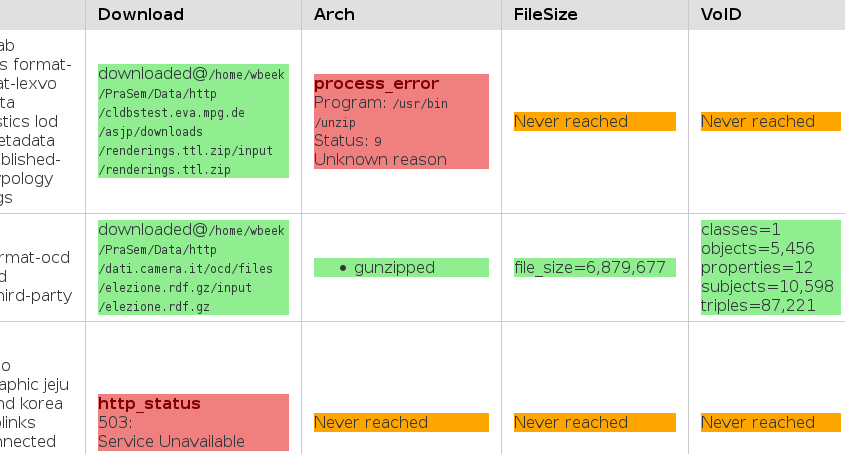
\includegraphics[width=0.85\textwidth]{./img/table}
  \caption{
    A part of the table that is generated by \obs.
    Each row in the table displays the results of retrieving a single
     resource from Datahub.
    Each column in the table corresponds to a specific action
     that is performed for a specific resource.
    The picture shows the results of executing the following four actions
     for three resources:
     (1) downloading the resource,
     (2) unarchiving it,
     (3) determining the file size, and
     (4) counting some basic VoID statistics \cite{Void2011}.
  }
\end{figure*}

\subsubsection*{Locating resources}

CKAN uses URLs as universal locators for resources.
URLs are URIs that identify a resource via a representation of
 its primary access mechanism or scheme (e.g. HTTP)
 and its network location (e.g. \texttt{www.datahub.io})
 that can be accessed using standardized operations
 defined for that scheme. \cite{Rfc3305}

The datasets that are catalogued by CKAN provide
 a starting point for an automated agent to search for data on the Web,
 since all data registrations can be queried using an API.
Since datasets have to be explicitly registered at a CKAN catalogue,
 this ensures that they are purposefully published
 as machine-processable data,
 thereby following our definition of a `resource'
 (see section \ref{sec:operationalization})
Each CKAN resource has a URL property field,
 which allows an automated agent to find a URL string for each resource.

\subsubsection*{Connecting to disseminating host}

When using the URL string to locate a resource we find that
 not all URL strings parse according to the grammar
 in the URL specification \cite{Rfc3986},
 and some URLs that are grammatically correct contain a scheme
 that is not registered with
 the Internet Assigned Numbers Authority
 (IANA).\footnote{\url{http://www.iana.org/assignments/uri-schemes/uri-schemes.xhtml}}
%\footnote{
%  The number of resources for which the URL string parses correctly
%  can be increased by trimming leading and trailing whitespace (US-ASCII 32)
%  and by prepending the string with a commonly occurring scheme descriptor
%  (e.g., \texttt{http://}) in case the grammar cannot detect a scheme.
%}

Culprits:
\begin{itemize}[noitemsep,nolistsep]
  \item The URL string does not parse according to the RFC grammar.
  \item The parsed URL string does not contain an IANA-registered scheme.
\end{itemize}

For URLs that are grammatically correct an automated agent is able to
 verify whether there exists a host authority at the location
 denoted by the URL.
As with the Web of Documents, this is not always the case,
 resulting in a ``host not found exception''.
Once a host authority is found, it has to accept a connection
 with the automated agent.
Only when a connection is established can the agent send its request
 to the authority.
The agent and authority both have to maintain the connection
 for the duration of the subsequent request/response-interaction.

Culprits:
\begin{itemize}[noitemsep,nolistsep]
\item The host that is denoted by the URL's authority string cannot be found.
\item The connection was refused by the host.
\item The connection was neither refused nor accepted by the host.
\item The connection was established, but was broken off
      during subsequent communication.
\item The host was redirecting the connecting agent indefinitely.
\end{itemize}

\subsubsection*{Retrieving resource from host}

Once a reliable connection between agent and host is established
 for the duration of a communicative interaction,
 the agent is able to send a request in one of
 the standardized Internet communication protocols.
Specifically, \obs supports communications via FTP and HTTP(S).

Various things can go wrong in both formulating the request and
 in replying to it.
This results in various status codes that denote different problems
 that cause the communication to be ineffective.

\subsubsection*{Open license}

Many CKAN registered resources have a license property.
The licenses are similar to those defined by the Open Data Commons,
 but some mismatches occur.
In the Datahub CKAN repository, 33 licenses are used,
 18 of which are underdefined (i.e., with no semantic description),
 impacting 5\% of the resources.
We have added manual mappings from the CKAN licenses onto
 the repository of Open Data Commons license descriptions.
%This results in added descriptions for 14 underdefined licenses,
% additional properties for 4 licenses that were already partially defined,
% and leaves only 2 underdefined licenses that have been equated to
% `license' \texttt{ckan:None} using \texttt{owl:sameAs} statements.

Culprits:
\begin{itemize}[noitemsep,nolistsep]
\item Has no license string.
\item Has a license string that cannot be mapped to
       a license that occurs in
       the Open Data Commons license description set.
\item Has a recognized license that is not open.
\end{itemize}

\subsubsection*{Structured \& non-propetary}
\label{sec:implementation_mime}

In order to implement the structuredness requirement,
 we have manually classified the MIME types that occur in the CKAN catalogue
 into `structured' and `unstructured' ones.
This goes against our interpretation of structuredness as
 a gradient property, but the partial order constituted by the relation
 ``supports at least the same set of relational operators''
 cannot be easily established in an automated way,
 as this would require a model of query operators
 and a description of MIME types in terms of the operators that are
 supported by those content types.

We list the 4 ways in which we can check for a resource's content type
 in CKAN, annotated with the number of resources for which
 this type can be retrieved:
\begin{itemize}[noitemsep,nolistsep]
  \item The value of the CKAN \texttt{mimetype} property.
        Present for 6,332 resources (45\%).
  \item The value of the CKAN \texttt{format} property
        Present for 10,226 resources (73\%).
  \item The MIME type in the HTTP \texttt{Content-Type} response header
         (not present in CKAN).
  \item The extension of the resource file.
\end{itemize}

We are specifically interested in linked data,
 but not all linked data serialization formats have a MIME type
 that is registered by IANA.
Moreover, some of the registered linked data content types are deprecated.
We take both deprecated and current MIME types into account,
 and officially registered ones as well as ones that are
 de facto being used to denoted linked data.
Not all MIME types that occur in CKAN repositories are valid,
 some of them seem to be typos/variants of existing MIME types
 for which we have added mappings manually.

The values of the CKAN \texttt{format} property are not standardized
 and are also manually mapped onto IANA-registered and de facto used
 MIME types.
Some of the format values seem to be typographic variants
 of each other (impacting 96 resources).
For some format values no mapping to an existing MIME type
 could be found (impacting 52 resources).

%The MIME type that occurs in the \texttt{Content-Type} response header
% is not always the same as the MIME type denoted by either the
% \texttt{format} or the \texttt{mimetype} property.
%Sometimes this is more generic or a more specific than
% the CKAN-registered value (XX\%),
% but sometimes it is another value altogether.

File extensions were not mapped to content type,
 because of the absence of a straightforward mapping.
We do not believe file extensions are a reliable indicator
 of a resource's format.

A special case occurs for resources that are compressed
 in some archive format.
For these neither MIME type, format, nor Content-Type header
 are indicative of the uncompressed content,
 so for these we have to rely on the file extension.

When none of the above enumerated methods works,
 we can try to parse a file's first few lines.
This is generally quite difficult because of the large number
 of different formats, encoding types, and syntactic error that may occur.
In the general case we are only able to make a best guess at
 a resource's format.

Culprits:
\begin{itemize}[noitemsep,nolistsep]
  \item The resource's type is not set.
  \item The resource's type is set, but it does not map to a MIME type
         that is registered by IANA and it is not one of the MIME types
         in the list of de facto used identifiers of LOD content.
  \item The resource's type can be mapped to an IANA-registered type
         or a de facto LOD type, but it does not denote structured data.
  \item The resource's type can be mapped to an IANA-registered type
         or a de facto LOD type, but it denotes a proprietary format.
\end{itemize}

\subsubsection*{Syntactic correctness: readable triples}

We use SWI-Prolog's Semweb library \cite{wielemaker2003}
 for loading the resources into a triple store.

The number of triples that can be loaded is often inconsistent with
 the value of the CKAN \texttt{size} property.\footnote{The CKAN
    \texttt{size} property is often taken to represent the actual number
    of triples in a dataset.
   For example, the famous visualizations of the LOD cloud make use of
    the values for this property.
   Our observatory shows that these visualizations are not always based
    on the correct numbers.}

Culprits:
\begin{itemize}[noitemsep,nolistsep]
  \item From the resource no triples can be read.
  \item From the resource some triples are read (syntax errors).
  \item From the resource all triples are read (no syntax error).
\end{itemize}


\section{Experimental Validation}
\label{sec:experiment}
\label{sec:experimental_design}
\label{sec:experimental_validation}

In order to subject our theory to an experimental test,
  we use the IIMB dataset\footnote{\URL{islab.di.unimi.it/iimb}}
  used in the instance matching track of the
  2012 Ontology Alignment Evaluation Initiative
  (OAEI)\footnote{\URL{oaei.ontologymatching.org}}.
This dataset consists of eighty ontologies $G_i$ (for $1 \leq i \leq 80$)
  that are linked to a single base ontology $G_0$.
The identity links between $G_0$ and $G_i$ are annotated with a
  confidence measure between $0.0$ and $1.0$.
A graph $G$ is the result of fully materializing the graph merge
  of $G_i$ (for some $1 \leq i \leq 80$) and $G_0$.
For each of these eighty linked ontologies a reference mapping is available.

In our experiment we ran separate tests for each of the $80$ datasets
  and took the average values for incremental reductions of
  random parts of the identity relations between $G_0$ and the $80$
  different $G_i$'s.
In other words: we deliberately make the identity relation incomplete.
We then calculate the rough set representation using this altered relation.
Subsequently ,we evaluate how many of the removed identity pairs occur in
  the higher approximation.
Our hypothesis is that the percentage of removed \emph{identity pairs}
  in the higher approximation is larger than the percentage of \emph{pairs}
  in the higher approximation.
If the hypothesis is validated, this indicates that
  calculating the rough set representation for a partial identity relation
  would indeed improve suggestions for extending that identity relation.

Since the data may contain noise, using precision degrees $0.0$ and $1.0$
  may be too strict. For this experiment we have set the boundaries
  to $0.05$ and $0.95$ respectively.

Figure \ref{fig:recall_quality} shows the different behaviors of the
  upper and lower approximations, with the upper approximation indeed
  having a dramatically higher recall than the lower approximation.

\begin{figure}
\centering
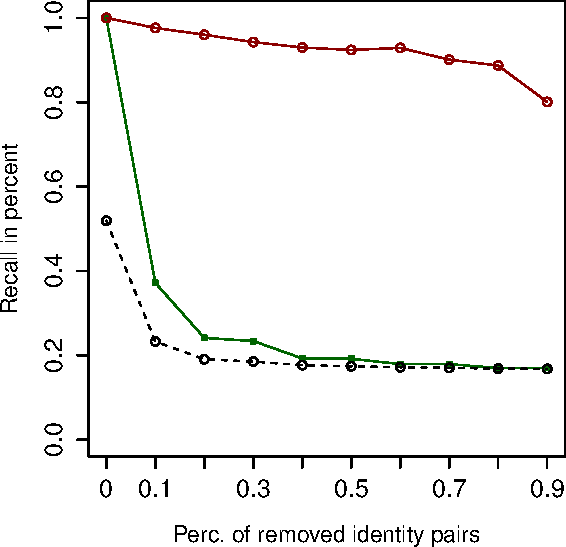
\includegraphics[width=0.8\linewidth]{./img/recall_quality}
\caption{
  The recall of the lower and higher approximation
    is shown by the green line (circles) and red line (boxes) respectively.
  The quality metric (definition \ref{def:quality})
    is shown by the dashed line.
}
\label{fig:recall_quality}
\end{figure}

In figure \ref{fig:in_higher}
  we see that the randomly removed identity pairs are often
  in the higher approximation, even when large parts of
  the identity relation are removed.

\begin{figure}
\centering
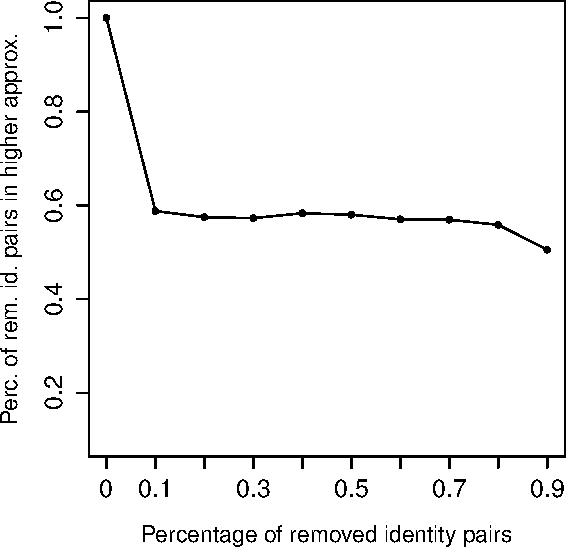
\includegraphics[width=0.8\linewidth]{./img/in_higher}
\caption{
  The percentage of the removed identity pairs that are in the higher approximation
}
\label{fig:in_higher}
\end{figure}

\begin{comment}
Lower recall
1.0,0.37172100183246687,0.24123550044617229,0.23375413992878838,0.19251810221158194,0.1916729296953922,0.1790536768898471,0.17912482945205316,0.1696252362320524,0.17011849853438268
Higher recall
1.0,0.976185052819561,0.9600384749021372,0.9425765362723856,0.9297564861502547,0.9239282325982691,0.9288077551757412,0.900878631549093,0.886987450993775,0.8005503359226204
Quality
0.5190405227795084,0.23261438049447705,0.1904353344556299,0.18505145463363135,0.17658153004935476,0.17387635867899948,0.17168948193128328,0.17017370794837366,0.16844506704419984,0.1677780567227606
Higher cover
0.0006413304103753317,0.0006098495555258293,0.0005825544051162525,0.0005747252831024628,0.0005640718998200667,0.0005626590987592347,0.0005613753926606205,0.0005464403973849621,0.0005372610299329459,0.00046916805031848495
Removed identity pairs in higher
1.0,0.5877680311890837,0.5747530425162004,0.572660333493667,0.5831761670185315,0.5799385908868745,0.5701984042084377,0.5692284399224807,0.558405393333526,0.5051324217787632
\end{comment}



\subsection{Future Experiments}
\label{sec:hypotheses}

Space limitations do not allow us to describe the results of further
  experiments. Instead, we will describe some of the other hypotheses
  that can be evaluated using our approach:
\begin{enumerate}
\item Take an {\small \texttt{owl:sameAs}} relation and
        a {\small \texttt{skos:related}}
        relation defined over the same domain.
      Merge them into a new binary relation $\sim$.
      Establishing the lower and higher approximation of $\sim$,
        the hypothesis is that pairs from {\small \texttt{owl:sameAs}}
        occur more frequently in the lower boundary than pairs from
        {\small \texttt{skos:related}},
\item Take a set of alignment pairs, each associated with a confidence measure
        between $0.0$ and $1.0$.
      Choose an arbitrary cutoff point $0.0 < c < 1.0$.
      The hypothesis is that alignments with a confidence larger than $c$
        occur more frequently in the lower approximation than alignments
        with a confidence smaller than $c$.
\item Take a set of automatically generated alignment pairs with
        associated confidence measures and take the gold standard or
        reference alignment for the same dataset.
      The hypothesis is that pairs that occur in the lower approximation
        of the alignment appear relatively more often in the gold standard
        than pairs that occur in the higher approximation of the alignment.
\item The quality measure $\alpha$ of a reference alignment is generally
        higher than the accuracy measure of an automatically generated
        alignment for the same dataset.
      Or, the quality measure is generally higher for identity relations
        that domain experts consider to be correct.
\end{enumerate}

\noindent Finally, the IIMB datasets are quite small
  (tens of thousands of triples).
We will have to verify whether the current implementation is able to scale
  to bigger datasets.


\section{Extensions}
\label{sec:extensions}

In section \ref{sec:approach} 
  we made some simplifications in order to keep the discussion brief.
We discuss three extensions to our base approach.
The first extension provides further details on how to assess
  identity conditions of typed literals, which may occur in the object
  position of a triple.
The second extension generalizes the notion of a
  predicate, allowing more indiscernibility predicates to be found.
The third extension shows that definitions
  \ref{def:identity_lower_approximation} and
  \ref{def:identity_higher_approximation}
  do not give the most optimal solution in some arcane cases.

\subsection{Identity of typed literals}

In order to deal with predefined datatypes such as integers, dates, etc.,
  RDF introduces the notion of ``typed literals''.
For such typed literals, identity does not suffice in order to ascertain
  that the sets of object terms denote the same resources
  (definition \ref{def:indiscernibility_properties}).
The reason for this is that typed literals have special identity conditions.
Since typed literals are quite common in SW data, we elaborate on this here.
Roughly speaking, for typed literals we assume a lexical-to-value mapping
  \cite{Hayes2004}, which assigns a value to each lexical expression.
For each datatype we assume a datatype-specific identity relation
  partitioning the datatype's value space.
Identity between typed literals is then defined
  as the datatype-specific identity between the values of the literals
  under the lexical-to-value mapping.
This extension was already used to perform the computational
  experiment of section \ref{sec:experiment}.

\begin{comment}
First we assume a datatype map
  \mbox{$D : \mathcal{I} \rightarrow ICEXT(I({\small \texttt{rdfs:Datatype}}))$},
  where $ICEXT$ is the functional map from classes onto their instances.
Second, for each datatype $d$ we assume a lexical-to-value mapping
  $L2V(d)$,\cite{Hayes2004},
  %: V(d) \rightarrow LEX(d)
  which assigns a value to each lexical expression.
Finally, for each datatype $d$ we assume a datatype-specific identity relation
  $\sim_d$ partitioning the datatype's value space $V(d)$.\footnote{
    Relation $\sim_d$ poses some problems to implement correctly,
      see section \ref{sec:implementation} for details.
    }

Suppose that two objects $o_1$ and $o_2$ are both typed literals,
  with $o_1 = \pair{d_1}{x_1}$ and $o_2 = \pair{d_2}{x_2}$
  for datatype names $d_1$ and $d_2$ and value names $x_1$ and $x_2$.
Identity between $o_1$ and $o_2$ is then defined as in
  \ref{def:identity_typed_literals}.

\begin{definition}[Identity for typed literals]
\label{def:identity_typed_literals}
\begin{align}
  o_1 \approx o_1
\,\iff\,
    D(d_1) = D(d_2)
  & \; \land \; &\nonumber\\
    x_1 \in LEX(d_1)
  & \; \land \; &\nonumber\\
    x_2 \in LEX(d_2)
  & \; \land \; &\nonumber\\
    l2v(D(d_1))(x_1) \sim_d l2v(D(d_2))(x_2)\nonumber
\end{align}
\end{definition}

\noindent Notice that the datatype-specific lexical-to-value mapping
  in definition \ref{def:identity_typed_literals} is relevant for
  the identification of identity,
  since two lexical expressions may map onto the same value
  according to one datatype but onto different values
  according to another.
An example of this are the lexical expressions $0.1$ and $0.10000000009$,
  which map to the same value according to datatype
  {\small \texttt{xsd:float}}
  but to different values according to datatype
  {\small \texttt{xsd:decimal}} \cite{Goldberg1991}.

In definition \ref{def:identity_typed_literals}
  the conjuncts which state that the value names belong to
  the respective lexical spaces may seem superfluous at first.
But for ill-typed literals,
  i.e. those whose value names do not belong to the lexical space of
  the specified datatype,
  the interpretation is not determined and they are only known to denote
  some arbitrary non-literal value \cite{Hayes2004}.\footnote{
    From the practice of working with SW data, the authors can testify
    that ill-typed literals do occur and are actually quite common!}
\end{comment}


\subsection{Path-expressions}
\label{sec:path_expressions}

The indiscernibility predicates in
  definition \ref{def:indiscernibility_predicates}
  were assumed to consist of single RDF predicate terms.
This restriction is rather arbitrary.
For instance,
  it may be the case that resources {\small \texttt{dbp:Amsterdam}}
  and {\small \texttt{openei:Amsterdam}} may not share a single property,
  even though the format is located in {\small \texttt{dbp:Netherlands}}
  and the latter is located in {\small \texttt{openei:Netherlands}}
  (but these are not asserted as being the same country).
However, suppose that {\small \texttt{dbp:Netherlands}}
  borders {\small \texttt{dbp:Germany}}
  and {\small \texttt{openei:Netherlands}}
  borders {\small \texttt{openei:Germany}},
  where {\small \texttt{dbp:Germany}} and
  {\small \texttt{openei:Germany}} are asserted to be identical.
If we generalize the notion of a predicate,
  then {\small \texttt{dbp:Amsterdam}} and
  {\small \texttt{openei:Amsterdam}} will share the property
  of being located in a country that borders Germany.
Obviously, Brussels and Brno share this property as well,
  so Brussels, Brno and Amsterdam will be indiscernible with respect to
  this predicate (taken in isolation), but the property is at least
  able to discern Brussels, Brno and Amsterdam from
  Stuttgart, Portland, and The Netherlands.

The notion of a predicate, can be easily generalized
  so that it can be denoted by a sequence of RDF predicate terms.
Such sequences are called \emph{path-expressions} in RDF. 

\begin{comment}
For each sequence of predicate terms $\tuplerange{p_1}{p_n}$
  we assume a functional mapping
  $f_{\tuplerange{p_1}{p_n}} : S_G \rightarrow \powerset{O_G}$,
  called the property sequence mapping
  \mbox{(definition \ref{def:generalized_property_map})}.

\begin{definition}[Property sequence map]
\label{def:generalized_property_map}
\begin{align}
  f_{\tuplerange{p_1}{p_n}}(s)
\,=\,
  \bigsetdef{o \in O_G}{
    \exists_{\range{x_0}{x_n}}(
      x_0 = s \land x_n = o \land\nonumber\\
      \bigwedge_{i=0}^{n-1}\nolimits
          \pair{I(x_i)}{I(x_{i+1})}
        \in
          \bigcup_{p \in \equivset{p_{i+1}}}\nolimits \mathit{Ext}(I(p))
    )
  }\nonumber
\end{align}
\end{definition}

By using property sequence maps,
  the definition for generalized indiscernibility predicates
  is only slightly more complex than its simplified version.

\begin{definition}[Indiscernibility criteria]
\label{def:indiscernibility_criteria}
\begin{align}
  \indp_{\approx}(\set{\range{x_1}{x_n}})
=
  \setdef{
    \tuplerange{p_1}{p_n} \in P_G^n
  }{\nonumber\\
      \exists \range{p_1^1}{p_1^n} \in \equivset{p_1},
    \ldots,
      \exists \range{p_m^1}{p_m^n} \in \equivset{p_n}
    (\nonumber\\
        \equivset{f_{\tuplerange{p_1^1}{p_m^1}} (x_1)}
      =
        \ldots
      =
        \equivset{f_{\tuplerange{p_1^n}{p_m^n}} (x_n)}
    )
  }\nonumber
\end{align}
\end{definition}
\end{comment}

\subsection{Fixpoint definition for approximations}

When using the definitions
  \ref{def:identity_lower_approximation} and
  \ref{def:identity_higher_approximation}
  for determining the rought set represention,
  we do not always get the most optimal solution.
We will illustrate this with the example depicted
  in figure \ref{fig:fixpoint}.

\begin{figure}
\label{fig:fixpoint}
\centering
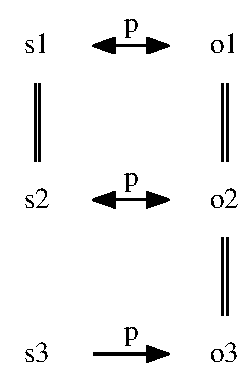
\includegraphics[width=0.4\columnwidth]{./img/fixpoint_example_cropped}
\caption{
  An illustrative example showing that defining
  $\lowerapprox$ in terms of $\higherapprox$ may not be optimal.
  The identity relation is represented with double-lined edges.
  $s_i$, $p$, and $o_i$ are subject, predicate, and object terms respectively.
  The directed edges represent triples.
}
\end{figure}

The indiscernibility criteria for this example are shown
  in equation \ref{eq:20}.

\begin{align}
\label{eq:20}
  \indp_{\approx}(\set{s_1,s_2,s_3})
&=\\
  \indp_{\approx}(\set{o_1,o_2})
&=
  \setdef{p^n}{\natnum{n}}\nonumber
\end{align}

\noindent Based on these indiscernibility criteria
  the naive lower approximation
  (definition \ref{def:identity_lower_approximation}) is empty.
But notice that there is a slight asymmetry in the way we have
  calculated this result.
We have defined $\lowerapprox$ in terms of $\indp_{\approx}$,
  i.e. in terms of $\approx$.
It seems more correct, however, to base the indiscernibility criteria
  for calculating the lower approximation on $\lowerapprox$ itself
  (and similarly for the higher approximation).
The resulting definition \ref{def:identity_lower_approximation_fixpoint}
  is recursive.
It affects the closure operations over the predicate and object terms
  in \mbox{definition \ref{def:indiscernibility_predicates}}.

\begin{definition}
\label{def:identity_lower_approximation_fixpoint}
\begin{align}
  x \in \lowerapprox
\, \iff \,
    \setdef{y}{x \equiv_{\indp_{\lowerapprox}} y}
  \; \subseteq \;
    \approx\nonumber
\end{align}
\end{definition}

\noindent There are now two correct solutions or fixpoints
  for the present example:

The first solution is the same as for the naive definition;
  $\lowerapprox_1 = \emptyset$,
  where $\indp_{\lowerapprox_1}(X) = \emptyset$
  for $X$ such that $\card{X} > 1$.

The second solution could not be derived in the naive case:
  $\lowerapprox_2 = \set{\pair{s_1}{s_2},\pair{o_1}{o_2}}$,
  with $\indp_{\lowerapprox_2}(\set{s_1,s_2,o_1,o_2}) = \setdef{p^n}{\natnum{n}}$
  and $\indp_{\lowerapprox_1}(X) = \emptyset$
  for all other $X$ such that $\card{X} > 1$.
This is the greatest fixpoint for this example.

Both solutions are correct,
  since both conform to the same strictures imposed by the here presented
  framework.
However, the second solution is better, since a greater fixpoint is
  to be prefered over a smaller fixpoint.
This is in line with our intuitions,
  since this enlarges the number of consistently applied identity pairs,
  as can be glanced from the quality criterion in
  \mbox{definition \ref{def:quality}}.
Reasoning along the same lines,
  a least fixpoint\footnote{
      We have no reason to believe that it should be unique.
    }
  is the best solution for the redefined higher approximation.




\section{Conclusion}
\label{sec:conclusion}

In this paper we presented a new approach for characterizing,
  extending, retracting, and assessing identity relations.
Our approach does this in purely qualitative terms, using schema semantics.

In section \ref{sec:introduction} we enumerated three research goals.
The first goal is met, since an indiscernibility partition characterizes
  identity subrelations based on the predicates $P$ (closed under identity)
  for which the pairs in that sets are indiscernible.
In this way we can distinguish between different types of identity
  by treating $P$ as a description of a (sub)set of identity pairs.
We suggest that the meaning of an identity relation and its subrelations
  is partially defined in its use,
  i.e., in the indiscernibility criteria it embodies.

The second goal is met, since the notion of a rough set allows us to
  distinguish between pairs that must be (lower approximation)
  and those that may be (higher approximation)
  % 'may' = 'not must not'
  in the identity relation.
If we want to add/remove pairs of the identity relation,
  we should not consider pairs of the former but only pairs of
  the latter kind.

The third goal is met, since the measure for rough set accuracy
  is based on the discernibility criteria of an identity set.
The crispness of the set is proportional to the quality of the
  identity relation, based on its semantic consistency.


%\input{./tex/futurework.tex}

% Bibliography
\bibliographystyle{aaai}
\bibliography{iotw,prasem,web_standards}

\end{document}

